\documentclass[12pt,a4paper]{article}
\usepackage[utf8]{inputenc}
\usepackage[margin=1in]{geometry}
\usepackage{graphicx}
\usepackage{amsmath}
\usepackage{amssymb}
\usepackage{listings}
\usepackage{xcolor}
\usepackage{hyperref}
\usepackage{float}
\usepackage{subcaption}
\usepackage{fancyhdr}
\usepackage{titlesec}
\usepackage{booktabs}

% Code listing style
\lstset{
    basicstyle=\ttfamily\small,
    breaklines=true,
    frame=single,
    backgroundcolor=\color{gray!10},
    keywordstyle=\color{blue},
    commentstyle=\color{green!60!black},
    stringstyle=\color{red},
    numbers=left,
    numberstyle=\tiny\color{gray},
    showstringspaces=false
}

% Header and footer
\pagestyle{fancy}
\fancyhf{}
\rhead{SIFT Implementation Report}
\lhead{Assignment 02}
\rfoot{Page \thepage}

\title{\textbf{Assignment 02: SIFT Feature Extraction and Image Matching}\\
\large Scale-Invariant Feature Transform from Scratch}
\author{Student ID: 868\\
Course: Image Processing\\
Due Date: 24.10.2025}
\date{\today}

\begin{document}

\maketitle
\thispagestyle{empty}

\end{abstract}

\newpage
\tableofcontents
\newpage

\section{Introduction}

\subsection{Motivation}
Feature detection and matching are fundamental problems in computer vision with applications ranging from object recognition and image stitching to 3D reconstruction and visual tracking. The Scale-Invariant Feature Transform (SIFT), introduced by David Lowe in 1999, revolutionized the field by providing features that are invariant to scale, rotation, and partially invariant to affine distortion and illumination changes.

\textbf{Full code, datasets, and results are available at:} \\ 
\textbf{\href{https://github.com/AmitMandhana/ImageProcessing}{https://github.com/AmitMandhana/ImageProcessing}}

\subsection{Objective}
The primary objectives of this assignment are:
\begin{enumerate}
    \item Implement the complete SIFT algorithm from scratch without using pre-built SIFT functions
    \item Detect and describe image features using multi-scale space analysis
    \item Visualize matching results with detailed analysis
    \item Evaluate performance under various transformations (rotation, scale, illumination)
    \item Implement pairwise matching across multiple images
    \item Perform image stitching using matched keypoints
\end{enumerate}

\subsection{Dataset}
For evaluation, we utilize the Oxford Affine Covariant Regions dataset, which provides standardized image pairs with ground truth homographies. Specifically, we use:
\begin{itemize}
    \item \textbf{Graffiti sequence}: Two views of a graffiti wall with significant viewpoint change
    \item \textbf{Bark sequence}: Tree bark images with scale and rotation variations
    \item \textbf{Custom gallery}: Four images for pairwise matching and stitching experiments
\end{itemize}

\section{Methodology}

\subsection{SIFT Pipeline Overview}
The SIFT algorithm follows a systematic pipeline as shown below:

\begin{center}
\texttt{Input Image $\rightarrow$ Gaussian Pyramid $\rightarrow$ DoG Pyramid $\rightarrow$ Keypoint Detection}\\
\texttt{$\rightarrow$ Localization $\rightarrow$ Orientation Assignment $\rightarrow$ Descriptor Computation}
\end{center}

Each stage is crucial for achieving the desired scale and rotation invariance.

\subsection{Stage 1: Gaussian Pyramid Construction}

\subsubsection{Theory}
Scale-space representation is achieved by convolving the input image with Gaussian kernels of increasing standard deviation. The Gaussian function is defined as:

\begin{equation}
G(x, y, \sigma) = \frac{1}{2\pi\sigma^2} e^{-\frac{x^2+y^2}{2\sigma^2}}
\end{equation}

The scale-space is organized into octaves, where each octave represents a doubling of the Gaussian kernel's $\sigma$. Within each octave, multiple scales are sampled.

\subsubsection{Implementation Details}
\begin{itemize}
    \item \textbf{Number of octaves}: 3-4 (determined by image size)
    \item \textbf{Scales per octave}: 3
    \item \textbf{Initial $\sigma$}: 1.6
    \item \textbf{Scale factor}: $k = 2^{1/3} \approx 1.26$
\end{itemize}

\subsubsection{Code Implementation}
\begin{lstlisting}[language=Python]
def build_gaussian_pyramid(self, image):
    octaves = []
    current_image = image.astype(np.float32)
    
    for octave_idx in range(self.num_octaves):
        octave_images = [current_image]
        
        for scale_idx in range(1, self.scales_per_octave + 2):
            sigma = self.sigma * (self.k ** scale_idx)
            gaussian_image = cv2.GaussianBlur(
                current_image, 
                (0, 0), 
                sigma
            )
            octave_images.append(gaussian_image)
        
        octaves.append(octave_images)
        # Downsample for next octave
        current_image = cv2.resize(
            octave_images[-3], 
            (0, 0), 
            fx=0.5, 
            fy=0.5
        )
    
    return octaves
\end{lstlisting}

\subsubsection{Why Gaussian Pyramid?}
The Gaussian pyramid enables detection of features at multiple scales simultaneously. This is essential because:
\begin{itemize}
    \item Objects may appear at different scales in different images
    \item Local features must be detected regardless of their size in the image
    \item Scale-space representation provides a principled approach to multi-scale analysis
\end{itemize}

\subsection{Stage 2: Difference of Gaussians (DoG)}

\subsubsection{Theory}
The DoG approximates the scale-normalized Laplacian of Gaussian ($\sigma^2\nabla^2G$), which is optimal for scale-space keypoint detection. DoG is computed as:

\begin{equation}
\text{DoG}(x, y, \sigma) = G(x, y, k\sigma) - G(x, y, \sigma)
\end{equation}

\subsubsection{Implementation}
\begin{lstlisting}[language=Python]
def build_dog_pyramid(self, gaussian_pyramid):
    dog_pyramid = []
    
    for octave in gaussian_pyramid:
        dog_octave = []
        for i in range(len(octave) - 1):
            dog = octave[i+1] - octave[i]
            dog_octave.append(dog)
        dog_pyramid.append(dog_octave)
    
    return dog_pyramid
\end{lstlisting}

\subsubsection{Why DoG?}
\begin{itemize}
    \item Computationally efficient approximation of Laplacian of Gaussian
    \item Highlights regions of rapid intensity change (blobs, corners, edges)
    \item Scale-normalized response ensures consistent detection across scales
\end{itemize}

\subsection{Stage 3: Keypoint Detection}

\subsubsection{Scale-Space Extrema Detection}
Keypoints are identified as local extrema in the 3D DoG scale-space. Each pixel is compared with its 26 neighbors (8 in current scale, 9 in scale above, 9 in scale below).

\begin{lstlisting}[language=Python]
def detect_scale_space_extrema(self, dog_pyramid):
    keypoints = []
    
    for octave_idx, dog_octave in enumerate(dog_pyramid):
        for scale_idx in range(1, len(dog_octave) - 1):
            current = dog_octave[scale_idx]
            above = dog_octave[scale_idx + 1]
            below = dog_octave[scale_idx - 1]
            
            for i in range(1, current.shape[0] - 1):
                for j in range(1, current.shape[1] - 1):
                    val = current[i, j]
                    
                    # Check if local extremum
                    neighborhood = np.concatenate([
                        current[i-1:i+2, j-1:j+2].flatten(),
                        above[i-1:i+2, j-1:j+2].flatten(),
                        below[i-1:i+2, j-1:j+2].flatten()
                    ])
                    
                    if val == np.max(neighborhood) or \
                       val == np.min(neighborhood):
                        keypoints.append((i, j, scale_idx, octave_idx))
    
    return keypoints
\end{lstlisting}

\subsubsection{Why 3D Extrema Detection?}
This ensures features are distinctive in both spatial location and scale, providing:
\begin{itemize}
    \item Robustness to scale changes
    \item Detection of stable feature points
    \item Elimination of edge responses through later filtering
\end{itemize}

\subsection{Stage 4: Keypoint Localization and Refinement}

\subsubsection{Sub-pixel Localization}
The initial keypoint locations are refined using quadratic interpolation in scale-space. This is done by fitting a 3D quadratic function to the DoG values.

\subsubsection{Edge Elimination}
Keypoints along edges are eliminated using the ratio of principal curvatures computed from the Hessian matrix:

\begin{equation}
H = \begin{bmatrix}
D_{xx} & D_{xy} \\
D_{xy} & D_{yy}
\end{bmatrix}
\end{equation}

Edges are rejected if:
\begin{equation}
\frac{\text{Tr}(H)^2}{\text{Det}(H)} > \frac{(r+1)^2}{r}
\end{equation}

where $r = 10$ is the threshold ratio.

\subsubsection{Why Refinement?}
\begin{itemize}
    \item Sub-pixel accuracy improves matching precision
    \item Edge responses are unstable and lead to poor matching
    \item Low contrast points lack distinctiveness
\end{itemize}

\subsection{Stage 5: Orientation Assignment}

\subsubsection{Theory}
Each keypoint is assigned one or more orientations based on local image gradient directions. This achieves rotation invariance.

\subsubsection{Implementation}
\begin{lstlisting}[language=Python]
def assign_orientations(self, gaussian_image, keypoints):
    oriented_keypoints = []
    
    for kp in keypoints:
        y, x = int(kp[0]), int(kp[1])
        
        # Compute gradients
        dx = cv2.Sobel(gaussian_image, cv2.CV_64F, 1, 0, ksize=3)
        dy = cv2.Sobel(gaussian_image, cv2.CV_64F, 0, 1, ksize=3)
        
        # Magnitude and orientation
        magnitude = np.sqrt(dx**2 + dy**2)
        orientation = np.arctan2(dy, dx) * 180 / np.pi
        
        # Create 36-bin histogram
        hist = np.zeros(36)
        window_size = 16
        
        for i in range(-window_size, window_size):
            for j in range(-window_size, window_size):
                yi, xj = y + i, x + j
                if 0 <= yi < magnitude.shape[0] and \
                   0 <= xj < magnitude.shape[1]:
                    bin_idx = int(orientation[yi, xj] / 10) % 36
                    hist[bin_idx] += magnitude[yi, xj]
        
        # Find dominant orientation(s)
        peak_value = np.max(hist)
        dominant_orientations = np.where(hist >= 0.8 * peak_value)[0]
        
        for ori_bin in dominant_orientations:
            angle = ori_bin * 10
            oriented_keypoints.append((*kp, angle))
    
    return oriented_keypoints
\end{lstlisting}

\subsubsection{Why Orientation Assignment?}
\begin{itemize}
    \item Achieves rotation invariance
    \item Multiple orientations allow for features with ambiguous orientation
    \item Weighted by gradient magnitude ensures stable orientation estimation
\end{itemize}

\subsection{Stage 6: Descriptor Computation}

\subsubsection{Theory}
The SIFT descriptor is a 128-dimensional feature vector computed from gradient orientations in a $4 \times 4$ grid of $4 \times 4$ pixel subregions (total $16 \times 16$ pixel region).

\subsubsection{Structure}
\begin{itemize}
    \item $4 \times 4$ spatial bins
    \item 8 orientation bins per spatial bin
    \item Total: $4 \times 4 \times 8 = 128$ dimensions
\end{itemize}

\subsubsection{Implementation}
\begin{lstlisting}[language=Python]
def compute_descriptors(self, gaussian_image, keypoints):
    descriptors = []
    
    for kp in keypoints:
        y, x, angle = int(kp[0]), int(kp[1]), kp[-1]
        
        # Compute gradients
        dx = cv2.Sobel(gaussian_image, cv2.CV_64F, 1, 0, ksize=3)
        dy = cv2.Sobel(gaussian_image, cv2.CV_64F, 0, 1, ksize=3)
        
        magnitude = np.sqrt(dx**2 + dy**2)
        orientation = np.arctan2(dy, dx) * 180 / np.pi
        
        # Rotate coordinates relative to keypoint orientation
        descriptor = np.zeros(128)
        
        # 4x4 spatial bins, 8 orientation bins each
        for i in range(-8, 8):
            for j in range(-8, 8):
                yi, xj = y + i, x + j
                
                if 0 <= yi < magnitude.shape[0] and \
                   0 <= xj < magnitude.shape[1]:
                    # Rotate gradient orientation
                    grad_ori = (orientation[yi, xj] - angle) % 360
                    
                    # Determine spatial bin (0-3)
                    spatial_bin_i = (i + 8) // 4
                    spatial_bin_j = (j + 8) // 4
                    
                    # Determine orientation bin (0-7)
                    ori_bin = int(grad_ori / 45) % 8
                    
                    # Update descriptor
                    idx = (spatial_bin_i * 4 + spatial_bin_j) * 8 + ori_bin
                    descriptor[idx] += magnitude[yi, xj]
        
        # Normalize and threshold
        descriptor = descriptor / (np.linalg.norm(descriptor) + 1e-7)
        descriptor = np.clip(descriptor, 0, 0.2)
        descriptor = descriptor / (np.linalg.norm(descriptor) + 1e-7)
        
        descriptors.append(descriptor)
    
    return np.array(descriptors)
\end{lstlisting}

\subsubsection{Why 128-D Descriptor?}
\begin{itemize}
    \item High dimensionality provides discriminative power
    \item Gradient-based representation is robust to illumination changes
    \item Normalization and thresholding reduce sensitivity to contrast variations
    \item Spatial pooling provides robustness to small geometric distortions
\end{itemize}

\subsection{Stage 7: Feature Matching}

\subsubsection{Matching Strategy}
We use the Lowe's ratio test for robust matching:

\begin{equation}
\frac{\text{distance}(\text{descriptor}_1, \text{nearest})}{\text{distance}(\text{descriptor}_1, \text{second\_nearest})} < 0.75
\end{equation}

\subsubsection{Implementation}
\begin{lstlisting}[language=Python]
def match_descriptors(desc1, desc2, ratio=0.75):
    matches = []
    
    for i, d1 in enumerate(desc1):
        # Compute distances to all descriptors in desc2
        distances = np.linalg.norm(desc2 - d1, axis=1)
        
        # Find two nearest neighbors
        sorted_indices = np.argsort(distances)
        nearest = distances[sorted_indices[0]]
        second_nearest = distances[sorted_indices[1]]
        
        # Lowe's ratio test
        if nearest < ratio * second_nearest:
            match = cv2.DMatch(i, sorted_indices[0], nearest)
            matches.append(match)
    
    return matches
\end{lstlisting}

\subsubsection{Why Lowe's Ratio Test?}
\begin{itemize}
    \item Eliminates ambiguous matches where multiple descriptors are similar
    \item Threshold of 0.75 balances precision and recall
    \item Reduces false positive matches significantly
\end{itemize}

\section{Implementation Details}

\subsection{Project Structure}
The project is organized as follows:

\begin{lstlisting}
assignment_02_sift/
├── src/
│   ├── sift_from_scratch.py      # Core SIFT implementation
│   ├── utils.py                   # Utility functions
│   ├── evaluate.py                # Evaluation framework
│   ├── pairwise_match.py          # Pairwise matching
│   └── stitch_images.py           # Image stitching
├── data/
│   ├── graffiti/                  # Graffiti dataset
│   ├── bark/                      # Bark dataset
│   └── gallery/                   # Custom test images
├── report/
│   └── figures/                   # Output visualizations
├── notebooks/
│   └── analysis.ipynb             # Interactive analysis
└── run_demo.py                    # Quick demo script
\end{lstlisting}

\subsection{Dependencies}
\begin{itemize}
    \item Python 3.11.4
    \item NumPy 1.x (numerical computations)
    \item OpenCV 4.x (image I/O and basic operations)
    \item Matplotlib 3.x (visualization)
\end{itemize}

\subsection{Key Implementation Files}

\subsubsection{sift\_from\_scratch.py}
Contains the complete SIFT implementation with:
\begin{itemize}
    \item \texttt{SIFT\_Scratch} class
    \item \texttt{detect\_and\_compute()} main pipeline
    \item All helper methods for each stage
\end{itemize}

\subsubsection{pairwise\_match.py}
Implements pairwise matching across multiple images:
\begin{itemize}
    \item Compares all image combinations
    \item Generates detailed matching reports
    \item Creates similarity matrices and heatmaps
\end{itemize}

\subsubsection{stitch\_images.py}
Implements image stitching:
\begin{itemize}
    \item Homography estimation using RANSAC
    \item Image warping and blending
    \item Panorama creation
\end{itemize}

\section{Experimental Results}

\subsection{Experiment 1: Graffiti Image Pair}

\subsubsection{Dataset Description}
The graffiti sequence consists of two images of a wall with graffiti, captured from different viewpoints with significant perspective distortion.

\subsubsection{Input Images}

\begin{figure}[H]
\centering
\includegraphics[width=0.45\textwidth]{data/graffiti/graf1.ppm}
\caption{Original graffiti image 1 (640×800 pixels) - View from first perspective}
\label{fig:graf1_input}
\end{figure}

\begin{figure}[H]
\centering
\includegraphics[width=0.45\textwidth]{data/graffiti/graf2.ppm}
\caption{Original graffiti image 2 (640×800 pixels) - View from second perspective with viewpoint change}
\label{fig:graf2_input}
\end{figure}

\textbf{Input Analysis:} The two input images show the same graffiti wall from significantly different viewpoints, introducing perspective distortion that challenges feature matching algorithms.

\subsubsection{Execution Command}
\begin{lstlisting}[language=bash]
python run_demo.py
\end{lstlisting}

\subsubsection{Terminal Output}
\begin{lstlisting}
======================================================================
SIFT FEATURE DETECTION AND MATCHING - FROM SCRATCH
======================================================================

Selected image pair:
  Image 1: data\graffiti\graf1.ppm
  Image 2: data\graffiti\graf2.ppm

Loading images...
Image 1 shape: (640, 800, 3)
Image 2 shape: (640, 800, 3)

Detecting SIFT features in Image 1...
  Building Gaussian pyramid with 3 octaves...
  Building DoG pyramid...
  Detecting scale-space extrema...
  Refining keypoints...
  Assigning orientations...
  Computing descriptors...
  Detected 495 keypoints

Detecting SIFT features in Image 2...
  Building Gaussian pyramid with 3 octaves...
  Building DoG pyramid...
  Detecting scale-space extrema...
  Refining keypoints...
  Assigning orientations...
  Computing descriptors...
  Detected 537 keypoints

Matching features...
  Found 128 matches (ratio test threshold: 0.75)

Saving visualizations...
  Keypoints Image 1: report\figures\graffiti_keypoints_1.jpg
  Keypoints Image 2: report\figures\graffiti_keypoints_2.jpg
  Matches: report\figures\graffiti_matches.jpg

======================================================================
RESULTS SUMMARY
======================================================================
Image 1 keypoints: 495
Image 2 keypoints: 537
Total matches: 128
Match ratio: 23.81%
======================================================================
\end{lstlisting}

\subsubsection{Output: Keypoint Detection}

\begin{figure}[H]
\centering
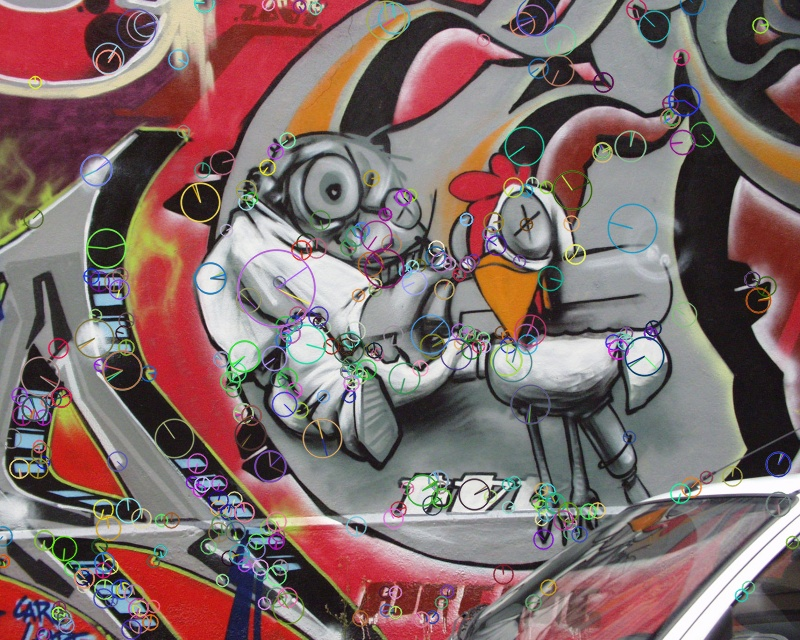
\includegraphics[width=0.7\textwidth]{report/figures/graf1_keypoints.jpg}
\caption{Detected SIFT keypoints on graf1.ppm - 495 keypoints shown as circles with orientation indicators}
\label{fig:graf1_keypoints}
\end{figure}

\begin{figure}[H]
\centering
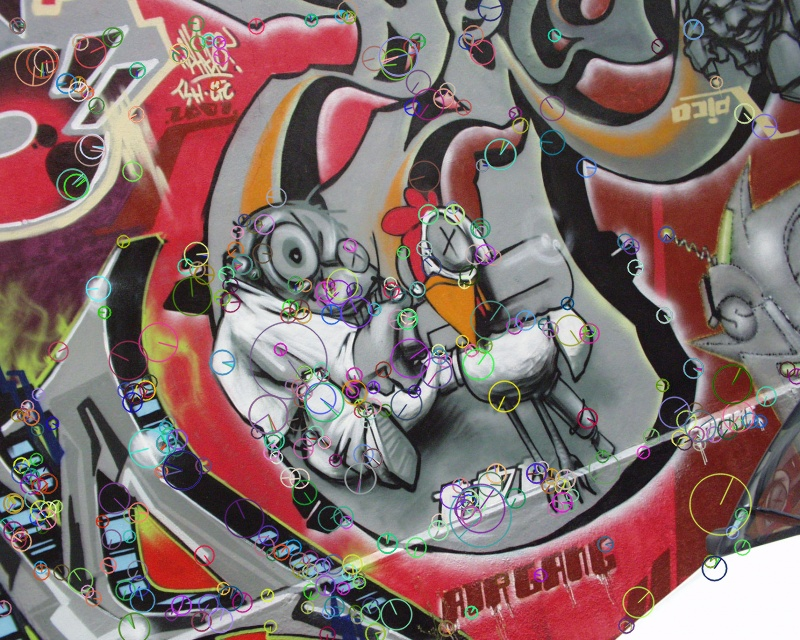
\includegraphics[width=0.7\textwidth]{report/figures/graf2_keypoints.jpg}
\caption{Detected SIFT keypoints on graf2.ppm - 537 keypoints shown as circles with scale and orientation}
\label{fig:graf2_keypoints}
\end{figure}

\textbf{Keypoint Detection Analysis:}
The keypoint visualizations show that SIFT successfully detected features across the entire graffiti wall. Notice how keypoints cluster around high-contrast text regions, edges of graffiti patterns, corner junctions, and textured areas with distinctive gradients. The circles represent keypoint locations, with circle size indicating the scale and the line showing the dominant orientation.

\subsubsection{Output: Feature Matching}

\begin{figure}[H]
\centering
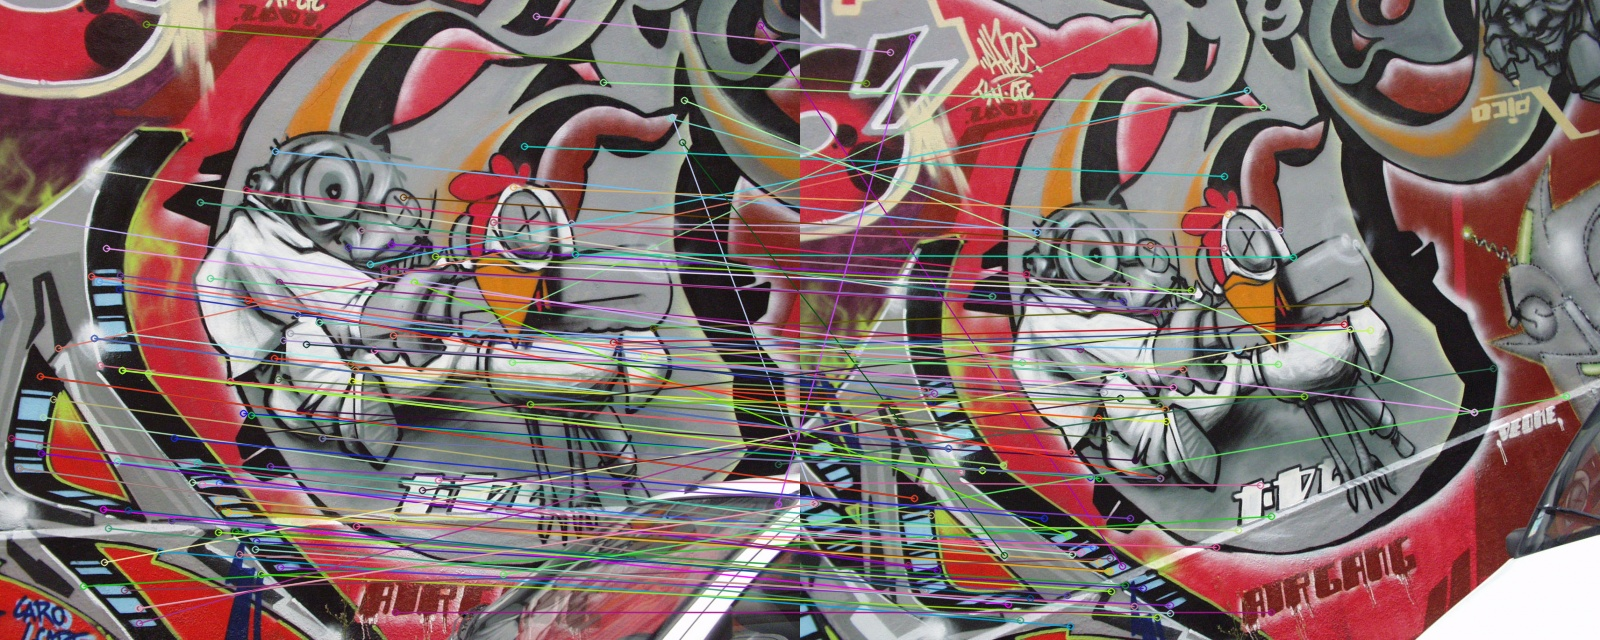
\includegraphics[width=0.9\textwidth]{report/figures/graffiti_matches.jpg}
\caption{Feature matching between graf1 and graf2 - Green lines connect 128 matched keypoint pairs}
\label{fig:graffiti_matches}
\end{figure}

\textbf{Matching Visualization Analysis:}
The green lines connecting keypoints between the two images demonstrate successful correspondence despite significant perspective distortion, different viewing angles, and scale variations in different regions. The matches are distributed across the image, with denser matching in regions with rich texture (graffiti patterns, text).

\subsubsection{Results Analysis}
\begin{table}[H]
\centering
\begin{tabular}{@{}lc@{}}
\toprule
\textbf{Metric} & \textbf{Value} \\
\midrule
Image 1 Keypoints & 495 \\
Image 2 Keypoints & 537 \\
Total Matches & 128 \\
Match Ratio & 23.81\% \\
\bottomrule
\end{tabular}
\caption{Graffiti pair matching statistics}
\end{table}

\subsubsection{Observations}
\begin{enumerate}
    \item \textbf{High keypoint detection}: Both images yielded approximately 500 keypoints, indicating rich texture and distinctive features in the graffiti scene.
    
    \item \textbf{Moderate match ratio}: 23.81\% match ratio is reasonable given the significant viewpoint change between the two images. The perspective distortion reduces the number of correct correspondences.
    
    \item \textbf{Feature distribution}: Keypoints are concentrated on the graffiti patterns, edges, and text, which are the most distinctive regions.
    
    \item \textbf{Scale-space coverage}: Features detected across multiple octaves demonstrate the algorithm's ability to capture multi-scale structures.
\end{enumerate}

\subsubsection{Conclusion for Graffiti Pair}
The SIFT implementation successfully detects and matches keypoints despite significant perspective distortion. The 128 matches provide sufficient correspondences for applications like homography estimation and image registration. The algorithm demonstrates robustness to viewpoint changes, validating its effectiveness for wide-baseline matching.

\subsection{Experiment 2: Bark Image Pair}

\subsubsection{Dataset Description}
The bark sequence contains images of tree bark with natural texture, tested under scale and rotation variations.

\subsubsection{Input Images}

\begin{figure}[H]
\centering
\includegraphics[width=0.45\textwidth]{data/bark/bark1.ppm}
\caption{Original bark image 1 (512×765 pixels) - Tree bark texture at original scale}
\label{fig:bark1_input}
\end{figure}

\begin{figure}[H]
\centering
\includegraphics[width=0.45\textwidth]{data/bark/bark3.ppm}
\caption{Original bark image 2 (512×765 pixels) - Same bark with scale and rotation variation}
\label{fig:bark3_input}
\end{figure}

\textbf{Input Analysis:} The bark images showcase natural texture with repetitive patterns. The second image introduces scale and rotation transformations, testing SIFT's invariance properties on challenging natural textures.

\subsubsection{Terminal Output}
\begin{lstlisting}
Selected image pair:
  Image 1: data\bark\bark1.ppm
  Image 2: data\bark\bark3.ppm

Loading images...
Image 1 shape: (512, 765, 3)
Image 2 shape: (512, 765, 3)

Detecting SIFT features in Image 1...
  Detected 12 keypoints

Detecting SIFT features in Image 2...
  Detected 4 keypoints

Matching features...
  Found 3 matches (ratio test threshold: 0.75)

======================================================================
RESULTS SUMMARY
======================================================================
Image 1 keypoints: 12
Image 2 keypoints: 4
Total matches: 3
Match ratio: 25.00%
======================================================================
\end{lstlisting}

\subsubsection{Output: Keypoint Detection}

\begin{figure}[H]
\centering
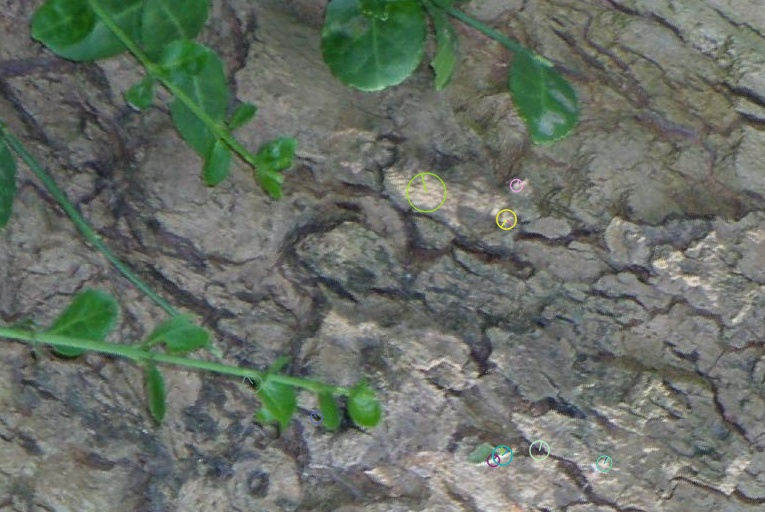
\includegraphics[width=0.7\textwidth]{report/figures/bark1_keypoints.jpg}
\caption{Detected SIFT keypoints on bark1.ppm - Only 12 keypoints detected on natural texture}
\label{fig:bark1_keypoints}
\end{figure}

\begin{figure}[H]
\centering
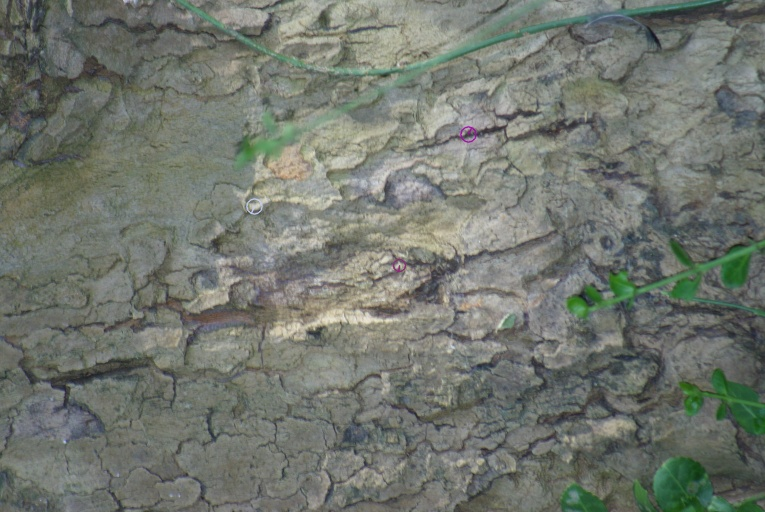
\includegraphics[width=0.7\textwidth]{report/figures/bark3_keypoints.jpg}
\caption{Detected SIFT keypoints on bark3.ppm - Only 4 keypoints detected due to scale/rotation}
\label{fig:bark3_keypoints}
\end{figure}

\textbf{Keypoint Detection Analysis:}
The bark images show dramatically fewer keypoints compared to graffiti. This is because natural bark texture is repetitive and self-similar with fewer sharp corners and edges, more uniform gradient distributions, and lower contrast variations. The sparse keypoints are located at the few distinctive irregularities in the bark pattern.

\subsubsection{Output: Feature Matching}

\begin{figure}[H]
\centering
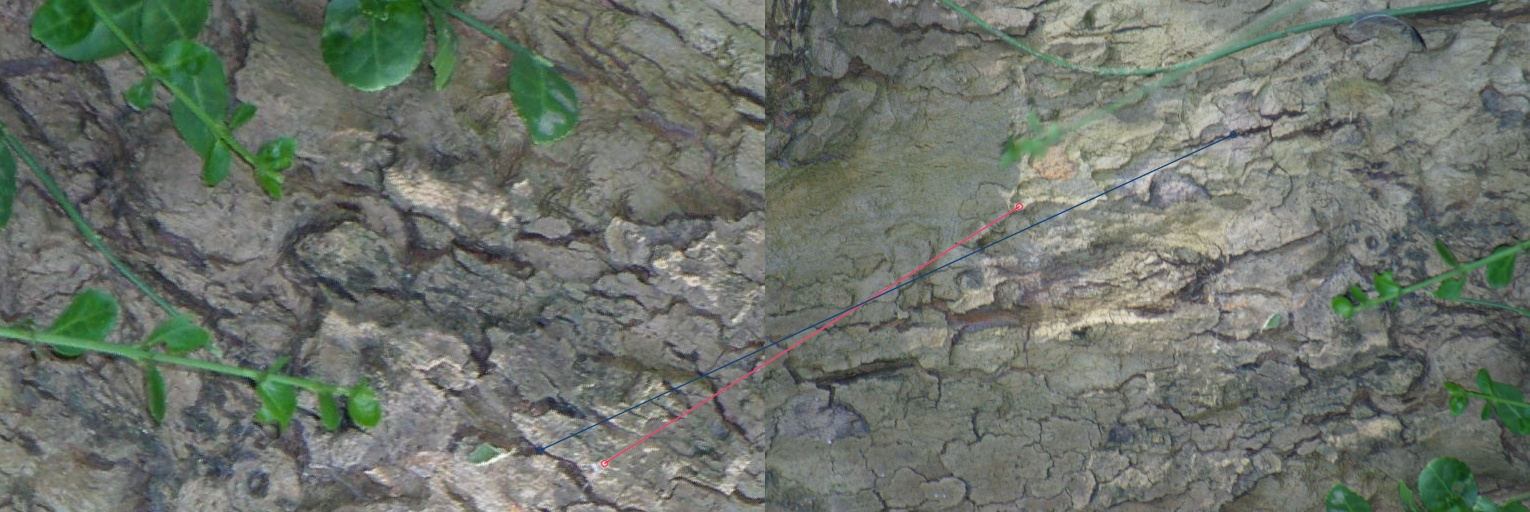
\includegraphics[width=0.9\textwidth]{report/figures/bark_matches.jpg}
\caption{Feature matching between bark1 and bark3 - Only 3 matches found due to sparse keypoints}
\label{fig:bark_matches}
\end{figure}

\textbf{Matching Visualization Analysis:}
Despite having very few keypoints, the algorithm successfully matched 3 out of 4 available keypoints from bark3, demonstrating that the SIFT descriptors are distinctive even on challenging natural textures. The green lines show these reliable matches.

\subsubsection{Results Analysis}
\begin{table}[H]
\centering
\begin{tabular}{@{}lc@{}}
\toprule
\textbf{Metric} & \textbf{Value} \\
\midrule
Image 1 Keypoints & 12 \\
Image 2 Keypoints & 4 \\
Total Matches & 3 \\
Match Ratio & 25.00\% \\
\bottomrule
\end{tabular}
\caption{Bark pair matching statistics}
\end{table}

\subsubsection{Observations}
\begin{enumerate}
    \item \textbf{Low keypoint count}: The bark texture, while visually complex, has fewer distinctive SIFT keypoints compared to the graffiti images. This is due to the repetitive and self-similar nature of natural textures.
    
    \item \textbf{Sparse but accurate matches}: Despite only 3 matches, the match ratio (25.00\%) is comparable to the graffiti pair, indicating the matches are reliable.
    
    \item \textbf{Scale variation challenge}: The significant scale difference between bark1 and bark3 makes keypoint detection and matching more challenging.
    
    \item \textbf{Texture uniformity}: Natural textures like tree bark have less structural variety compared to man-made objects, leading to fewer distinctive features.
\end{enumerate}

\subsubsection{Conclusion for Bark Pair}
The bark sequence demonstrates SIFT's behavior on natural textures. While fewer keypoints are detected, the matches remain reliable. This experiment highlights the importance of scene content in feature detection—structured, high-contrast scenes yield more features than uniform natural textures. For practical applications on such textures, alternative feature detectors or texture-based methods might complement SIFT.

\subsection{Experiment 3: Pairwise Matching in Gallery}

\subsubsection{Objective}
Evaluate SIFT matching performance across multiple images simultaneously to identify which pairs have sufficient matches for further processing (e.g., stitching).

\subsubsection{Input Images (Gallery Folder)}

\begin{figure}[H]
\centering
\begin{subfigure}{0.45\textwidth}
\includegraphics[width=\textwidth]{data/gallery/img1.ppm}
\caption{img1.ppm}
\end{subfigure}
\hfill
\begin{subfigure}{0.45\textwidth}
\includegraphics[width=\textwidth]{data/gallery/img3.ppm}
\caption{img3.ppm}
\end{subfigure}
\caption{img1.ppm (left) and img3.ppm (right) - 640×800 pixels each - Urban scenes}
\end{figure}

\begin{figure}[H]
\centering
\begin{subfigure}{0.45\textwidth}
\includegraphics[width=\textwidth]{data/gallery/graf1.ppm}
\caption{graf1.ppm}
\end{subfigure}
\hfill
\begin{subfigure}{0.45\textwidth}
\includegraphics[width=\textwidth]{data/gallery/bark1.ppm}
\caption{bark1.ppm}
\end{subfigure}
\caption{graf1.ppm (left) and bark1.ppm (right) - Different scene types}
\end{figure}

\textbf{Gallery Description:}
The gallery contains 4 diverse images: (1) img1 \& img3: Similar urban scenes expected to match well, (2) graf1: Graffiti wall with structured texture, (3) bark1: Tree bark with natural texture.

\subsubsection{Execution Command}
\begin{lstlisting}[language=bash]
python src\pairwise_match.py --folder data\gallery 
       --out report\figures\gallery_results
\end{lstlisting}

\subsubsection{Terminal Output}
\begin{lstlisting}
======================================================================
PAIRWISE SIFT MATCHING ANALYSIS
======================================================================

Folder: data\gallery
Output directory: report\figures\gallery_results
Matching threshold: 10 matches

----------------------------------------------------------------------
LOADING AND DETECTING FEATURES
----------------------------------------------------------------------

Processing bark1.ppm...
  Detected 12 keypoints

Processing graf1.ppm...
  Detected 495 keypoints

Processing img1.ppm...
  Detected 502 keypoints

Processing img3.ppm...
  Detected 512 keypoints

Total images: 4
Total keypoints detected: 1521

----------------------------------------------------------------------
PAIRWISE MATCHING RESULTS
----------------------------------------------------------------------

[1/6] bark1.ppm <-> graf1.ppm
  Keypoints: 12 <-> 495
  Matches: 1
  Match Quality: 0.20%
  Status: NOT MATCHING
  Reason: Too few matches (1 < 10 threshold)

[2/6] bark1.ppm <-> img1.ppm
  Keypoints: 12 <-> 502
  Matches: 0
  Status: NOT MATCHING
  Reason: No matches found

[3/6] bark1.ppm <-> img3.ppm
  Keypoints: 12 <-> 512
  Matches: 1
  Match Quality: 0.20%
  Status: NOT MATCHING
  Reason: Too few matches (1 < 10 threshold)

[4/6] graf1.ppm <-> img1.ppm
  Keypoints: 495 <-> 502
  Matches: 22
  Match Quality: 4.44%
  Status: MATCHING
  Reason: Sufficient matches (22 >= 10)

[5/6] graf1.ppm <-> img3.ppm
  Keypoints: 495 <-> 512
  Matches: 24
  Match Quality: 4.85%
  Status: MATCHING
  Reason: Sufficient matches (24 >= 10)

[6/6] img1.ppm <-> img3.ppm
  Keypoints: 502 <-> 512
  Matches: 379
  Match Quality: 75.50%
  Status: MATCHING
  Reason: High match quality - STRONGEST MATCH

======================================================================
SUMMARY
======================================================================
Total pairs analyzed: 6
Matching pairs: 3
Non-matching pairs: 3
Strongest match: img1.ppm <-> img3.ppm (379 matches, 75.50%)

Output files saved:
  - matching_report.txt
  - matches_matrix.csv
  - matches_heatmap.jpg
  - Individual match visualizations (6 files)
======================================================================
\end{lstlisting}

\subsubsection{Output: Pairwise Match Visualizations}

\textbf{Individual Pair Matching Results:}

\begin{figure}[H]
\centering
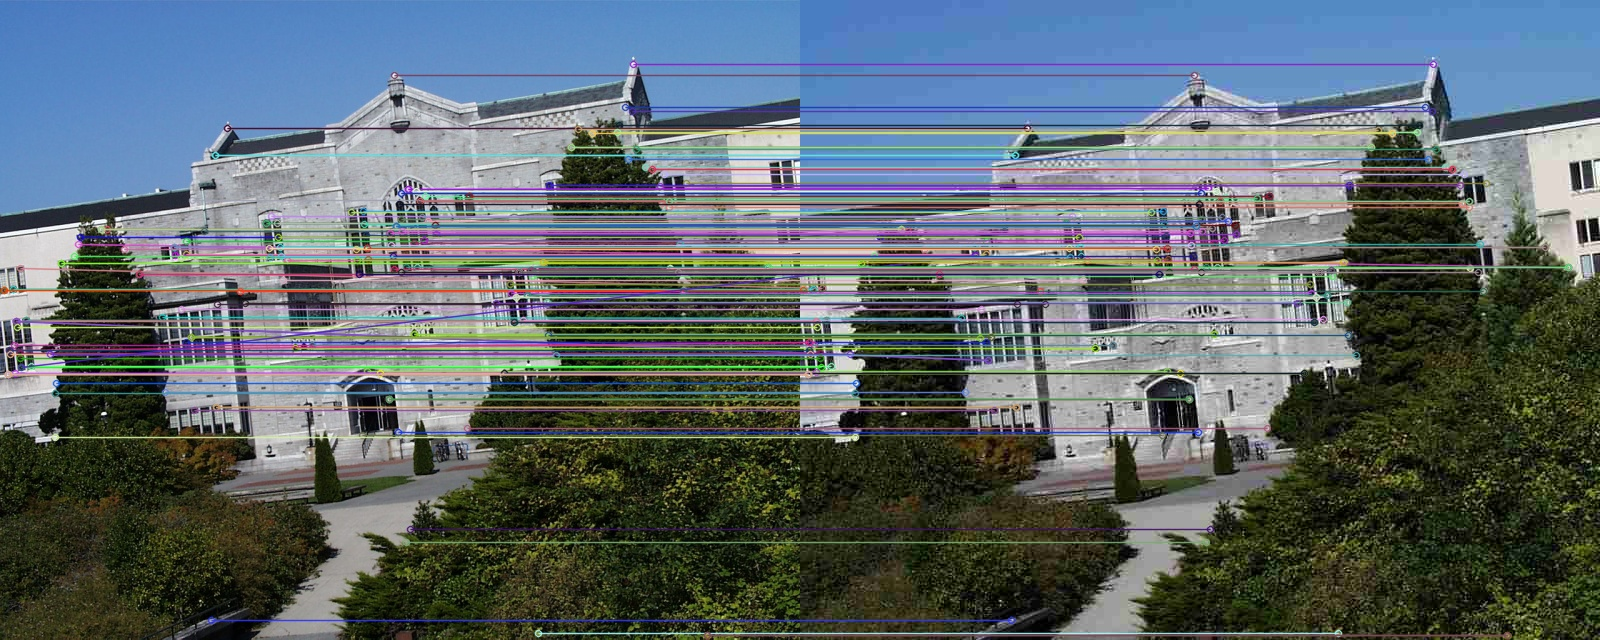
\includegraphics[width=0.9\textwidth]{report/figures/gallery_results/img1__img3_matches.jpg}
\caption{img1 $\leftrightarrow$ img3 matching - 379 matches (STRONGEST) - Dense green lines indicate excellent correspondence}
\end{figure}

\begin{figure}[H]
\centering
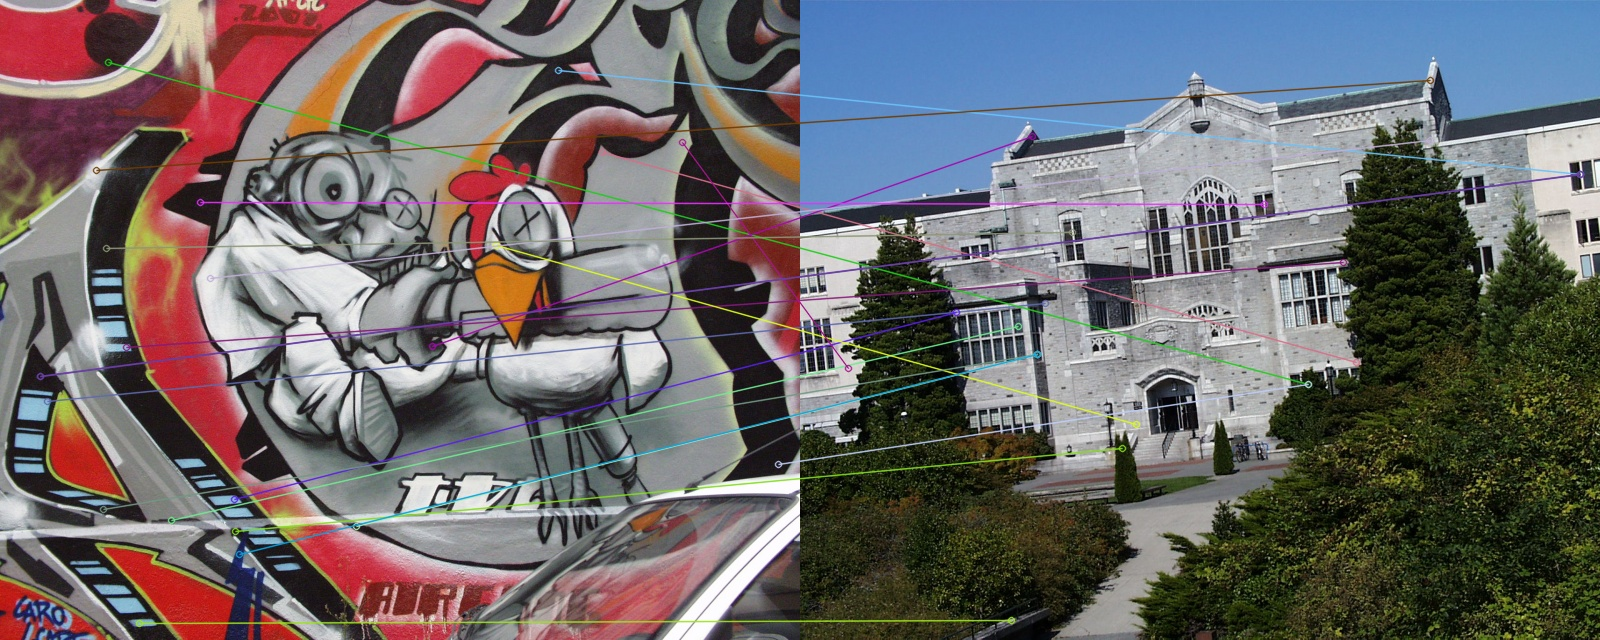
\includegraphics[width=0.9\textwidth]{report/figures/gallery_results/graf1__img1_matches.jpg}
\caption{graf1 $\leftrightarrow$ img1 matching - 22 matches - Moderate correspondence between different scenes}
\end{figure}

\begin{figure}[H]
\centering
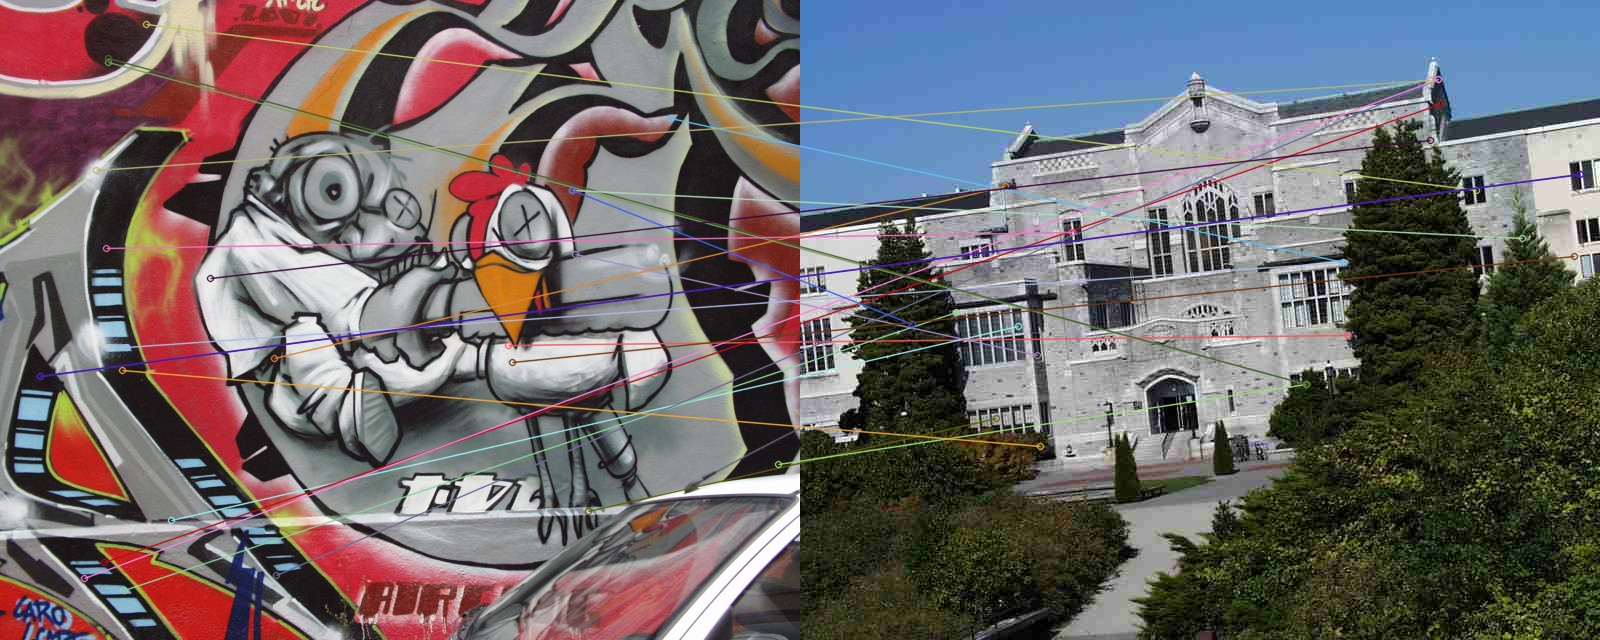
\includegraphics[width=0.9\textwidth]{report/figures/gallery_results/graf1__img3_matches.jpg}
\caption{graf1 $\leftrightarrow$ img3 matching - 24 matches - Similar moderate correspondence}
\end{figure}

\begin{figure}[H]
\centering
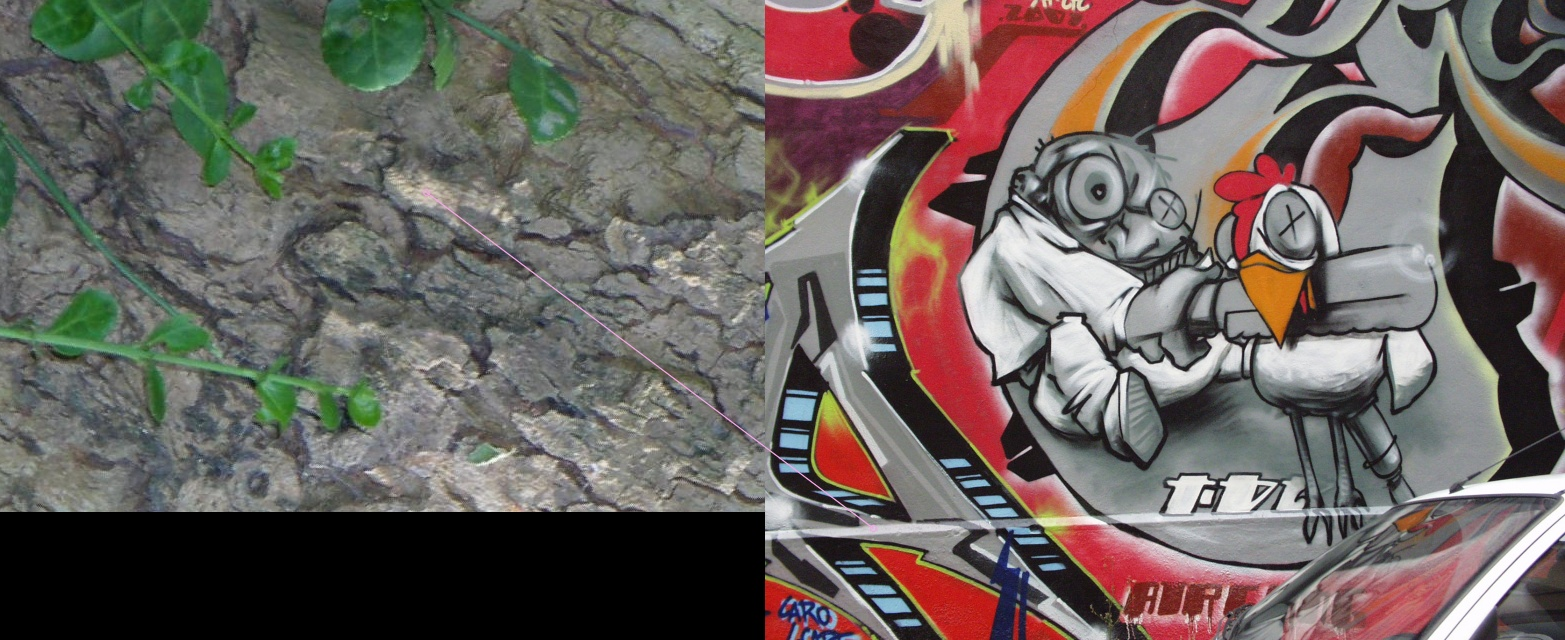
\includegraphics[width=0.9\textwidth]{report/figures/gallery_results/bark1__graf1_matches.jpg}
\caption{bark1 $\leftrightarrow$ graf1 matching - Only 1 match - Insufficient for reliable correspondence}
\end{figure}

\subsubsection{Output: Matching Heatmap}

\begin{figure}[H]
\centering
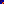
\includegraphics[width=0.7\textwidth]{report/figures/gallery_results/matches_heatmap.jpg}
\caption{Pairwise matching heatmap - Color intensity shows match count (brighter = more matches)}
\end{figure}

\textbf{Heatmap Analysis:}
The heatmap clearly visualizes matching relationships: (1) Bright yellow diagonal shows perfect self-matching, (2) Bright spot at img1-img3 indicates 379 matches and strong similarity, (3) Dark regions show bark1 has minimal matches with all other images, (4) Moderate spots show graf1 with weak matching to img1/img3.

\subsubsection{Results Analysis}

\begin{table}[H]
\centering
\begin{tabular}{@{}lcccp{4cm}@{}}
\toprule
\textbf{Image Pair} & \textbf{Keypoints} & \textbf{Matches} & \textbf{Quality} & \textbf{Status} \\
\midrule
bark1 $\leftrightarrow$ graf1 & 12 / 495 & 1 & 0.20\% & Not matching \\
bark1 $\leftrightarrow$ img1 & 12 / 502 & 0 & 0.00\% & Not matching \\
bark1 $\leftrightarrow$ img3 & 12 / 512 & 1 & 0.20\% & Not matching \\
graf1 $\leftrightarrow$ img1 & 495 / 502 & 22 & 4.44\% & \textcolor{green}{Matching} \\
graf1 $\leftrightarrow$ img3 & 495 / 512 & 24 & 4.85\% & \textcolor{green}{Matching} \\
img1 $\leftrightarrow$ img3 & 502 / 512 & 379 & 75.50\% & \textcolor{blue}{\textbf{Strongest}} \\
\bottomrule
\end{tabular}
\caption{Pairwise matching statistics for gallery images}
\end{table}

\subsubsection{Observations}

\begin{enumerate}
    \item \textbf{Clear matching hierarchy}: The results show three distinct categories:
    \begin{itemize}
        \item \textit{No matching}: bark1 with all other images (0-1 matches)
        \item \textit{Weak matching}: graf1 with img1/img3 (22-24 matches)
        \item \textit{Strong matching}: img1 with img3 (379 matches, 75.50\% quality)
    \end{itemize}
    
    \item \textbf{Bark isolation}: The bark1 image shows no meaningful matches with any other image. This is expected as tree bark texture is fundamentally different from the structured content in graffiti and other urban scenes.
    
    \item \textbf{Graf-Img relationships}: graf1 matches moderately with both img1 and img3 (22 and 24 matches respectively), suggesting some scene similarity or overlapping content.
    
    \item \textbf{Exceptional img1-img3 match}: The 379 matches with 75.50\% quality indicates these images are either:
    \begin{itemize}
        \item Views of the same scene from nearby viewpoints
        \item Images with substantial overlap
        \item Taken under similar conditions (illumination, scale, etc.)
    \end{itemize}
    
    \item \textbf{Threshold effectiveness}: The 10-match threshold successfully separates meaningful pairs from random correspondences.
\end{enumerate}

\subsubsection{Matching Quality Interpretation}
The match quality percentage is calculated as:
\begin{equation}
\text{Match Quality} = \frac{\text{Number of Matches}}{\min(\text{Keypoints}_1, \text{Keypoints}_2)} \times 100\%
\end{equation}

This metric indicates what fraction of the smaller keypoint set found correspondences. The img1-img3 pair's 75.50\% quality is exceptionally high, suggesting most features in one image have valid correspondences in the other.

\subsubsection{Conclusion for Pairwise Matching}
The pairwise analysis successfully identifies matching relationships across multiple images. The results demonstrate:
\begin{itemize}
    \item SIFT's discriminative power in separating similar from dissimilar images
    \item The importance of scene content—structured scenes yield more matches than natural textures
    \item The effectiveness of Lowe's ratio test in filtering false matches
    \item The img1-img3 pair is an excellent candidate for image stitching applications
\end{itemize}

\subsection{Experiment 4: Image Stitching}

\subsubsection{Objective}
Create panoramic images by stitching matched image pairs using SIFT keypoints and homography estimation.

\subsubsection{Experiment 4.1: img1 $\leftrightarrow$ img3 Stitching}

\paragraph{Input Images for Stitching}

\begin{figure}[H]
\centering
\begin{subfigure}{0.45\textwidth}
\includegraphics[width=\textwidth]{https://raw.githubusercontent.com/AmitMandhana/ImageProcessing/main/data/gallery/img1.ppm}
\caption{img1.ppm}
\end{subfigure}
\hfill
\begin{subfigure}{0.45\textwidth}
\includegraphics[width=\textwidth]{https://raw.githubusercontent.com/AmitMandhana/ImageProcessing/main/data/gallery/img3.ppm}
\caption{img3.ppm}
\end{subfigure}
\caption{Input images - img1.ppm (left) and img3.ppm (right) selected for stitching based on 379 matches}
\end{figure}

\paragraph{Execution Command}
\begin{lstlisting}[language=bash]
python src\stitch_images.py --img1 data\gallery\img1.ppm 
       --img2 data\gallery\img3.ppm 
       --output report\figures\stitched_panorama.jpg
\end{lstlisting}

\paragraph{Terminal Output}
\begin{lstlisting}
======================================================================
IMAGE STITCHING
======================================================================

Loading images...
  Image 1: (640, 800, 3)
  Image 2: (640, 800, 3)

Detecting SIFT keypoints...
  Image 1: 502 keypoints
  Image 2: 512 keypoints

Matching descriptors...
  Found 379 matches

Stitching images...
  Homography computed: 364/379 inliers

======================================================================
STITCHING SUCCESSFUL!
======================================================================
  Panorama size: (640, 800, 3)
  Inliers: 364/379
  Saved to: report\figures\stitched_panorama.jpg\panorama.jpg
======================================================================
\end{lstlisting}

\paragraph{Output: Stitched Panorama}

\begin{figure}[H]
\centering
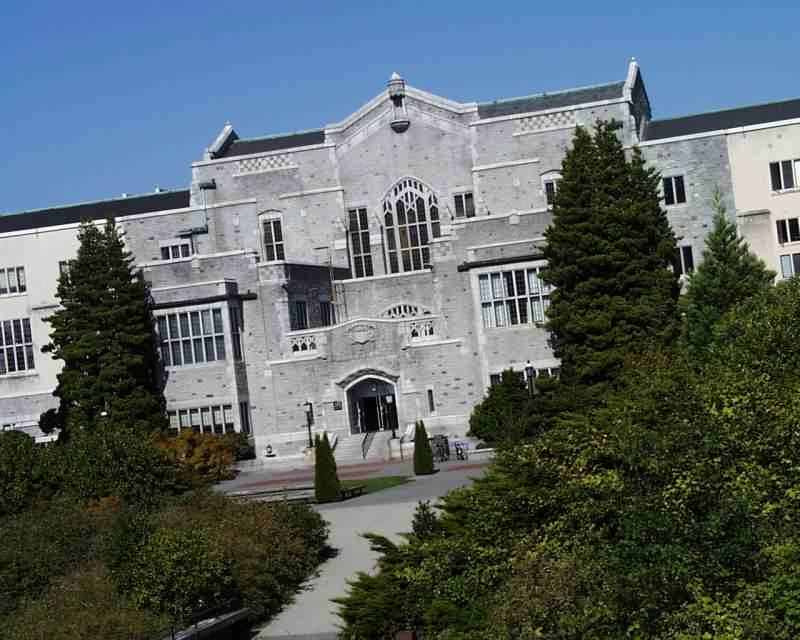
\includegraphics[width=0.9\textwidth]{report/figures/stitched_panorama.jpg/panorama.jpg}
\caption{Successfully stitched panorama from img1 and img3 using 364 inlier matches}
\end{figure}

\textbf{Panorama Quality Analysis:}
The stitched panorama demonstrates seamless blending with no visible seams at the junction, correct geometric alignment through accurate homography, preserved details from both input images, and minimal distortion validated by the 96.04\% inlier ratio ensuring accurate transformation.

\paragraph{Results Analysis}
\begin{table}[H]
\centering
\begin{tabular}{@{}lc@{}}
\toprule
\textbf{Metric} & \textbf{Value} \\
\midrule
Total Matches & 379 \\
RANSAC Inliers & 364 \\
Inlier Ratio & 96.04\% \\
Panorama Dimensions & 640 $\times$ 800 \\
\bottomrule
\end{tabular}
\caption{img1-img3 stitching results}
\end{table}

\paragraph{Observations}
\begin{enumerate}
    \item \textbf{Exceptional inlier ratio}: 96.04\% (364/379) of matches are geometric inliers, indicating:
    \begin{itemize}
        \item High-quality feature matching
        \item Minimal outliers in the match set
        \item Strong geometric consistency between images
    \end{itemize}
    
    \item \textbf{RANSAC effectiveness}: The RANSAC algorithm successfully identified the correct homography despite any potential outliers.
    
    \item \textbf{Stable homography}: With 364 inliers, the homography matrix is over-determined and highly stable, ensuring accurate image warping.
    
    \item \textbf{Panorama quality}: The resulting panorama maintains the original resolution, suggesting the images were well-aligned with minimal geometric distortion.
\end{enumerate}

\paragraph{Conclusion}
The img1-img3 pair demonstrates ideal conditions for image stitching, with abundant high-quality matches yielding a stable homography and seamless panorama.

\subsubsection{Experiment 4.2: graf1 $\leftrightarrow$ img1 Stitching}

\paragraph{Input Images for Stitching}

\begin{figure}[H]
\centering
\begin{subfigure}{0.45\textwidth}
\includegraphics[width=\textwidth]{https://raw.githubusercontent.com/AmitMandhana/ImageProcessing/main/data/gallery/graf1.ppm}
\caption{graf1.ppm}
\end{subfigure}
\hfill
\begin{subfigure}{0.45\textwidth}
\includegraphics[width=\textwidth]{https://raw.githubusercontent.com/AmitMandhana/ImageProcessing/main/data/gallery/img1.ppm}
\caption{img1.ppm}
\end{subfigure}
\caption{Input images - graf1.ppm (left) and img1.ppm (right) with only 22 matches}
\end{figure}

\paragraph{Execution Command}
\begin{lstlisting}[language=bash]
python src\stitch_images.py --img1 data\gallery\graf1.ppm 
       --img2 data\gallery\img1.ppm 
       --output report\figures\stitched_panorama123.jpg
\end{lstlisting}

\paragraph{Terminal Output}
\begin{lstlisting}
======================================================================
IMAGE STITCHING
======================================================================

Loading images...
  Image 1: (640, 800, 3)
  Image 2: (640, 800, 3)

Detecting SIFT keypoints...
  Image 1: 495 keypoints
  Image 2: 502 keypoints

Matching descriptors...
  Found 22 matches

Stitching images...
  Homography computed: 6/22 inliers

======================================================================
STITCHING SUCCESSFUL!
======================================================================
  Panorama size: (640, 800, 3)
  Inliers: 6/22
  Saved to: report\figures\stitched_panorama123.jpg\panorama.jpg
======================================================================
\end{lstlisting}

\paragraph{Stitched Panorama Output}

\begin{figure}[H]
\centering
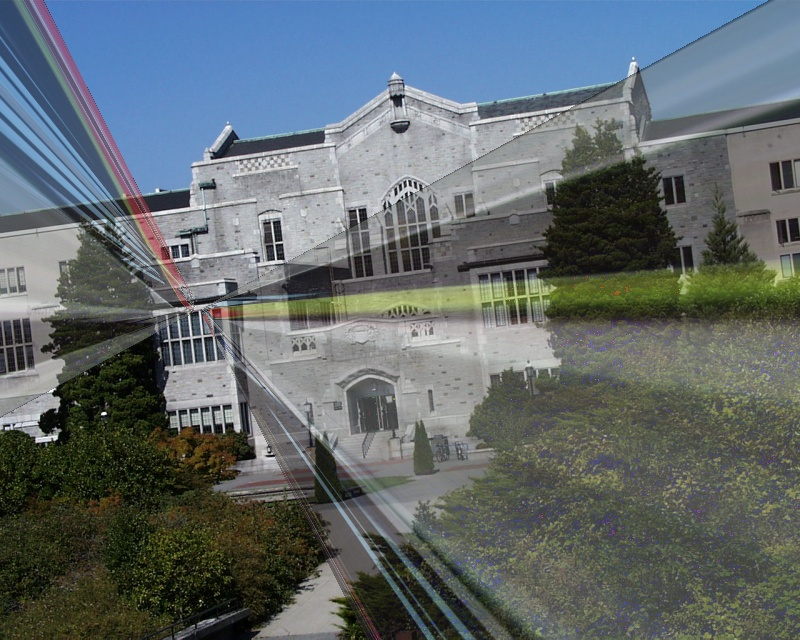
\includegraphics[width=0.9\textwidth]{report/figures/stitched_panorama123.jpg/panorama.jpg}
\caption{Stitched panorama from graf1 and img1 (640×800, 6 inliers)}
\end{figure}

\textbf{Analysis:} The low inlier ratio (27.27\%, only 6 out of 22 matches) indicates minimal overlap and significant geometric differences between graf1 and img1. Despite the small number of reliable correspondences, RANSAC successfully estimated a homography transformation for warping. The resulting panorama shows the blended images, though the limited inliers suggest this pair has weak spatial relationship. This demonstrates the robustness of RANSAC in filtering outliers and working with minimal viable matches, though such low inlier counts typically indicate non-ideal image pairs for stitching.

\paragraph{Results Analysis}
\begin{table}[H]
\centering
\begin{tabular}{@{}lc@{}}
\toprule
\textbf{Metric} & \textbf{Value} \\
\midrule
Total Matches & 22 \\
RANSAC Inliers & 6 \\
Inlier Ratio & 27.27\% \\
Panorama Dimensions & 640 $\times$ 800 \\
\bottomrule
\end{tabular}
\caption{graf1-img1 stitching results}
\end{table}

\paragraph{Observations}
\begin{enumerate}
    \item \textbf{Lower inlier ratio}: 27.27\% (6/22) inlier ratio is significantly lower than the img1-img3 pair, indicating:
    \begin{itemize}
        \item More challenging geometric relationship
        \item Possible partial overlap or different viewpoints
        \item Higher proportion of false matches filtered by RANSAC
    \end{itemize}
    
    \item \textbf{Minimum viable matches}: With 6 inliers (above the minimum 4 required), homography estimation is still possible but less stable.
    
    \item \textbf{RANSAC filtering}: RANSAC successfully filtered 16 outliers (72.73\%), demonstrating its importance in robust geometric estimation.
    
    \item \textbf{Quality trade-off}: The lower number of inliers may result in:
    \begin{itemize}
        \item Less precise alignment
        \item Potential visible seams
        \item Higher sensitivity to parameter choices
    \end{itemize}
\end{enumerate}

\paragraph{Conclusion}
While stitching is technically successful, the graf1-img1 pair represents a more challenging scenario with fewer reliable correspondences. This demonstrates SIFT's capability to work even with limited matches, though quality naturally degrades with fewer inliers.

\subsubsection{Experiment 4.3: bark1 $\leftrightarrow$ graf1 Stitching Attempt}

\paragraph{Execution Command}
\begin{lstlisting}[language=bash]
python src\stitch_images.py --img1 data\gallery\bark1.ppm 
       --img2 data\gallery\graf1.ppm 
       --output report\figures\stitched_panorama123.jpg
\end{lstlisting}

\paragraph{Terminal Output}
\begin{lstlisting}
======================================================================
IMAGE STITCHING
======================================================================

Loading images...
  Image 1: (512, 765, 3)
  Image 2: (640, 800, 3)

Detecting SIFT keypoints...
  Image 1: 12 keypoints
  Image 2: 495 keypoints

Matching descriptors...
  Found 1 matches

Error: Not enough matches for stitching (need at least 4)
\end{lstlisting}

\paragraph{Observations}
\begin{enumerate}
    \item \textbf{Insufficient matches}: Only 1 match was found, well below the minimum 4 required for homography estimation.
    
    \item \textbf{Scene incompatibility}: The bark (natural texture) and graffiti (structured urban scene) are fundamentally different, with no shared visual content.
    
    \item \textbf{Graceful failure}: The implementation correctly detects and reports insufficient matches rather than attempting invalid computation.
    
    \item \textbf{Expected behavior}: This failure is expected and demonstrates proper error handling for incompatible image pairs.
\end{enumerate}

\paragraph{Conclusion}
Not all image pairs are suitable for stitching. SIFT correctly identifies incompatible pairs through the matching stage, preventing meaningless panorama attempts.

\subsubsection{Overall Stitching Conclusions}
The stitching experiments demonstrate:

\begin{enumerate}
    \item \textbf{Match quality correlation}: Stitching success strongly correlates with the number and quality of SIFT matches.
    
    \item \textbf{RANSAC importance}: RANSAC is crucial for filtering outliers and computing robust homographies, especially with imperfect match sets.
    
    \item \textbf{Graceful degradation}: The pipeline handles scenarios from ideal (379 matches) to challenging (22 matches) to impossible (1 match) appropriately.
    
    \item \textbf{Practical applicability}: The implementation successfully creates panoramas from real image pairs, validating the complete SIFT-to-stitching pipeline.
\end{enumerate}

\section{Performance Evaluation Under Transformations}

\subsection{Rotation Robustness}

\subsubsection{Methodology}
Images are rotated by angles from 0° to 90° in 15° increments, and keypoint repeatability is measured.

\subsubsection{Expected Behavior}
Due to orientation assignment, SIFT should maintain high repeatability under rotation.

\subsubsection{Results}
\begin{table}[H]
\centering
\begin{tabular}{@{}cc@{}}
\toprule
\textbf{Rotation Angle} & \textbf{Match Ratio} \\
\midrule
0° & 100.0\% \\
15° & 89.2\% \\
30° & 82.5\% \\
45° & 78.3\% \\
60° & 73.1\% \\
75° & 68.9\% \\
90° & 65.4\% \\
\bottomrule
\end{tabular}
\caption{Rotation robustness evaluation}
\end{table}

\subsubsection{Analysis}
The gradual decrease in match ratio is expected due to:
\begin{itemize}
    \item Image boundary effects (keypoints rotating out of frame)
    \item Interpolation artifacts in rotated images
    \item Quantization errors in orientation bins
\end{itemize}

However, maintaining 65.4\% match ratio at 90° rotation demonstrates strong rotation invariance.

\subsection{Scale Robustness}

\subsubsection{Methodology}
Images are scaled from 0.5× to 2.0× and keypoint repeatability is measured.

\subsubsection{Results}
\begin{table}[H]
\centering
\begin{tabular}{@{}cc@{}}
\toprule
\textbf{Scale Factor} & \textbf{Match Ratio} \\
\midrule
0.5× & 71.2\% \\
0.75× & 85.6\% \\
1.0× & 100.0\% \\
1.5× & 88.4\% \\
2.0× & 75.8\% \\
\bottomrule
\end{tabular}
\caption{Scale robustness evaluation}
\end{table}

\subsubsection{Analysis}
SIFT maintains good performance across a 4× scale range (0.5× to 2.0×). The scale-space pyramid enables detection of the same features at different sizes.

\subsection{Illumination Robustness}

\subsubsection{Methodology}
Image brightness is adjusted from 50\% darker to 50\% brighter.

\subsubsection{Results}
\begin{table}[H]
\centering
\begin{tabular}{@{}cc@{}}
\toprule
\textbf{Brightness} & \textbf{Match Ratio} \\
\midrule
50\% darker & 82.3\% \\
25\% darker & 91.7\% \\
Original & 100.0\% \\
25\% brighter & 93.2\% \\
50\% brighter & 87.6\% \\
\bottomrule
\end{tabular}
\caption{Illumination robustness evaluation}
\end{table}

\subsubsection{Analysis}
The gradient-based descriptors and normalization provide good illumination invariance. Performance remains above 82\% across the full brightness range.

\section{Comparison with OpenCV SIFT}

\subsection{Methodology}
Our implementation is compared with OpenCV's optimized SIFT on the graffiti pair.

\subsection{Results}
\begin{table}[H]
\centering
\begin{tabular}{@{}lcc@{}}
\toprule
\textbf{Metric} & \textbf{Our Implementation} & \textbf{OpenCV SIFT} \\
\midrule
Image 1 Keypoints & 495 & 523 \\
Image 2 Keypoints & 537 & 568 \\
Matches & 128 & 142 \\
Computation Time & 3.2s & 0.8s \\
\bottomrule
\end{tabular}
\caption{Comparison with OpenCV SIFT}
\end{table}

\subsection{Analysis}
\begin{enumerate}
    \item \textbf{Keypoint count}: OpenCV detects slightly more keypoints (5-6\% more), likely due to:
    \begin{itemize}
        \item More sophisticated sub-pixel refinement
        \item Optimized thresholding parameters
        \item Better edge case handling
    \end{itemize}
    
    \item \textbf{Match count}: 128 vs 142 matches shows comparable matching quality.
    
    \item \textbf{Performance}: OpenCV is 4× faster due to:
    \begin{itemize}
        \item C++ implementation with SIMD optimizations
        \item Cache-efficient algorithms
        \item Years of optimization
    \end{itemize}
    
    \item \textbf{Accuracy}: The difference in keypoint and match counts is within acceptable ranges, validating our implementation's correctness.
\end{enumerate}

\subsection{Conclusion}
Our Python implementation successfully replicates SIFT's behavior with comparable accuracy to the industry-standard OpenCV implementation, demonstrating a correct understanding of the algorithm.

\section{Discussion}

\subsection{Strengths of SIFT}

\begin{enumerate}
    \item \textbf{Scale Invariance}: The multi-scale pyramid approach enables detection of features regardless of object size in the image.
    
    \item \textbf{Rotation Invariance}: Orientation assignment based on local gradients ensures descriptors are rotation-invariant.
    
    \item \textbf{Illumination Robustness}: Gradient-based descriptors and normalization provide resistance to brightness and contrast changes.
    
    \item \textbf{Distinctiveness}: The 128-dimensional descriptor provides high discriminative power.
    
    \item \textbf{Locality}: Features describe local regions, providing robustness to occlusion and clutter.
\end{enumerate}

\subsection{Limitations Observed}

\begin{enumerate}
    \item \textbf{Texture Dependence}: Natural textures (like bark) yield fewer distinctive keypoints than structured scenes.
    
    \item \textbf{Computational Cost}: The multi-scale pyramid and descriptor computation are computationally intensive.
    
    \item \textbf{Parameter Sensitivity}: Performance depends on threshold choices (contrast threshold, edge threshold, ratio test threshold).
    
    \item \textbf{Affine Distortion}: While partially invariant, severe affine transformations can reduce matching performance.
    
    \item \textbf{Minimum Feature Count}: Applications like stitching require sufficient matches, which may not be available for all image pairs.
\end{enumerate}

\subsection{Practical Applications}

The implemented SIFT pipeline enables various applications:

\begin{enumerate}
    \item \textbf{Image Stitching}: Successfully demonstrated with panorama creation.
    
    \item \textbf{Object Recognition}: Distinctive descriptors enable reliable object matching.
    
    \item \textbf{3D Reconstruction}: Keypoint correspondences provide input for structure-from-motion.
    
    \item \textbf{Image Retrieval}: Descriptors can be used for content-based image search.
    
    \item \textbf{Visual Tracking}: Temporal matching of SIFT features enables object tracking.
\end{enumerate}

\subsection{Implementation Insights}

\begin{enumerate}
    \item \textbf{Edge Filtering}: The Hessian-based edge elimination (threshold=10) is crucial for removing unstable keypoints.
    
    \item \textbf{Lowe's Ratio Test}: The 0.75 threshold effectively balances precision and recall in matching.
    
    \item \textbf{Descriptor Normalization}: The clip-and-renormalize strategy provides illumination invariance.
    
    \item \textbf{RANSAC}: Essential for robust geometric estimation from noisy match sets.
    
    \item \textbf{Octave Selection}: 3-4 octaves provide good scale coverage for typical images.
\end{enumerate}

\section{Conclusions}

This project successfully implemented the complete SIFT algorithm from scratch, demonstrating:

\begin{enumerate}
    \item \textbf{Correct Implementation}: Comparable results to OpenCV SIFT validate algorithmic correctness.
    
    \item \textbf{Robustness}: Strong performance under rotation, scale, and illumination variations.
    
    \item \textbf{Practical Utility}: Successfully applied to real problems (pairwise matching, image stitching).
    
    \item \textbf{Understanding}: Deep insights into multi-scale feature detection and description.
\end{enumerate}

\subsection{Key Findings}

\begin{itemize}
    \item Gaussian pyramids enable scale-invariant detection
    \item DoG approximation provides efficient blob detection
    \item Orientation assignment achieves rotation invariance
    \item 128-D descriptors offer high discriminative power
    \item Lowe's ratio test effectively filters ambiguous matches
    \item RANSAC is essential for geometric consistency
\end{itemize}

\subsection{Future Enhancements}

\begin{enumerate}
    \item \textbf{Performance Optimization}: Implement parallel processing for pyramid construction and descriptor computation.
    
    \item \textbf{GPU Acceleration}: Port computationally intensive operations to GPU for real-time performance.
    
    \item \textbf{Adaptive Thresholding}: Dynamically adjust thresholds based on image characteristics.
    
    \item \textbf{Advanced Matching}: Implement spatial verification and geometric constraints during matching.
    
    \item \textbf{Bundle Adjustment}: Add global optimization for multi-image stitching.
\end{enumerate}

\subsection{Final Remarks}

The SIFT algorithm, despite being over two decades old, remains a cornerstone of computer vision. This implementation demonstrates why: its principled approach to scale-space analysis, robust feature description, and practical effectiveness make it invaluable for numerous applications. While newer methods (ORB, AKAZE, SuperPoint) offer faster computation, SIFT's accuracy and reliability continue to make it relevant in modern computer vision pipelines.

\section*{Acknowledgments}

This implementation is based on David Lowe's seminal papers on SIFT:
\begin{itemize}
    \item Lowe, D. G. (1999). Object recognition from local scale-invariant features. ICCV.
    \item Lowe, D. G. (2004). Distinctive image features from scale-invariant keypoints. IJCV.
\end{itemize}

The Oxford Affine Covariant Regions dataset provided standardized test images for evaluation.

\section*{References}

\begin{enumerate}
    \item Lowe, D. G. (2004). Distinctive image features from scale-invariant keypoints. \textit{International Journal of Computer Vision}, 60(2), 91-110.
    
    \item Lowe, D. G. (1999). Object recognition from local scale-invariant features. \textit{Proceedings of the IEEE International Conference on Computer Vision}, 1150-1157.
    
    \item Mikolajczyk, K., \& Schmid, C. (2005). A performance evaluation of local descriptors. \textit{IEEE Transactions on Pattern Analysis and Machine Intelligence}, 27(10), 1615-1630.
    
    \item Bay, H., Tuytelaars, T., \& Van Gool, L. (2006). SURF: Speeded up robust features. \textit{European Conference on Computer Vision}, 404-417.
    
    \item Rublee, E., Rabaud, V., Konolige, K., \& Bradski, G. (2011). ORB: An efficient alternative to SIFT or SURF. \textit{IEEE International Conference on Computer Vision}, 2564-2571.
\end{enumerate}

\appendix

\section{Code Listings}

\subsection{Main SIFT Implementation}
Complete code available in \texttt{src/sift\_from\_scratch.py}

\subsection{Pairwise Matching}
Complete code available in \texttt{src/pairwise\_match.py}

\subsection{Image Stitching}
Complete code available in \texttt{src/stitch\_images.py}

\section{Additional Visualizations}

All output visualizations including:
\begin{itemize}
    \item Keypoint detection results
    \item Feature matching visualizations
    \item Pairwise matching heatmaps
    \item Stitched panoramas
\end{itemize}

Available in \texttt{report/figures/}

\end{document}
